\documentclass[a4paper,11pt]{article}
\usepackage[paper=a4paper,left=25mm,right=25mm,top=25mm,bottom=25mm]{geometry}
\usepackage{natbib}
\usepackage{graphicx}
\usepackage{amsmath}
\usepackage{gensymb}
\usepackage[usenames,dvipsnames]{xcolor}
\usepackage{setspace}
\usepackage{wrapfig}
\setcounter{secnumdepth}{-1}


\title{Forecasting cherry blossom blooms in 4 cities}
% \title{Different vibe: Blooms by biologists, how we see the next decade} 
% \title{}
% \title{}
% \title{}
% \title{}


\author{Tad Dallas,
Grant Foster,
Lauren Holian,
Robert Richards,
Cleber Ten Caten}
% authors in alphabetical order currently. Happy to change it up. Might just toss myself (TAD) as last author since I didn't do a whole lot. 

\date{\textit{Authors are listed alphabetically in author list}}


\begin{document}

\maketitle



\setstretch{1.3}


\subsubsection{Our motivations for joining this predictive challenge}

To a lab composed of theory-minded ecologists, the peak bloom prediction challenge represented a chance for some to leverage their quantitative skills, others, a time to navigate new territory in machine learning, and for all, an opportunity to explore the biology of an iconic species. However, though we could all envision the morphology of a cherry blossom, none of us would claim to be a botanist. As a result our approach was statistical in nature, we incorporated insights from the cherry blossom literature into a variety of relevant statistical models, each with their own strengths and weaknesses.



\subsubsection{How do we pick the most informative variables to include?}

Even the most flexible modeling framework will not be predictive without informative covariates. In a forecasting challenge such as this, we are intrinsically limited in the available feature space, as we do not only need covariate data for the existing data, but also in the future. We used predicted climate data from the CNRM-CM6-1 models available in the sixth phase of the Coupled Model Intercomparison Project (CMIP6) obtained from the copernicus database (\url{https://cds.climate.copernicus.eu/}) whereas past climate data was obtained from the National Oceanic and Atmospheric Administration (NOAA; \url{https://www.ncei.noaa.gov/access/search/}). Thus, for both past and future predictions, we obtained daily data for maximum temperature, minimum temperature and precipitation. We engineered covariates based on these three variables in three groups; 1) number of days above or below different thresholds for maximum and minimum temperature, 2) first day above or below threshold, and 3) number of consecutive days above or below threshold (Table \ref{tab:vars}). These temperature thresholds were selected because number of warm and cool days directly affects the blooming phenology of cherries. For example, a large number of cool days will delay the cherry blossom whereas cherry blossom will usually occur after a certain number of warm days is reached. 



\paragraph*{}
Our approach of focusing on temperature thresholds was inspired by previous work predicting cherry blooming dates using more mechanistic models. In chilling and forcing models constructed in the style of Jung et al. \cite{jung2005predicting}, the number of days spent below a given chilling threshold in the preceding fall or winter followed by the number of days spent above a second warming threshold the following spring together predict blossom bloom.  Therefore, we created features informed by a range of temperature thresholds, from as low as -2 $^{\circ}$C to as high as 25 $^{\circ}$C. We created features based not only on the total number of days above or below a certain threshold, but also longest stretch of consecutive days, or the earliest day in a given period to meet a given threshold. We created similar features looking both across the entire time series as well as within specific months we felt may be especially important for prediction. While having so many different temperature thresholds values makes optimization of any one particular impractical, we believe the fact that our machine learning approaches are able to leverage information from this large range of values while still being relatively robust to collinearity makes this trade-off worthwhile. In addition to climate features, we also include the site-level factors species-identity, latitude, and longitude, all of which likely capture additional site-level variation, such as differences in the definition of a ``bloom day''. Year is also included in an effort to capture any important long-term trends that our climate features may be missing. 






\begin{table}[h!]
\begin{center}
    \caption{Covariates used in predictive models of cherry blossom bloom date. }
	\vspace{0.5cm}
	\begin{tabular}{lll}
	 \hline
    Variable group & Condition & Threshold values or range \\
 	\hline
 	Number of days & $T_{max}$ $<$ threshold & 0,5,10,20,25 \\
 	& $T_{min}$ $<$ threshold & 0,5,8,10 \\
 	& $T_{max}$ $>$ 0 & month-specific (Dec, Jan, Feb) \\
    & Precipitation $>$ threshold & 0 \\ 	
 	& Precipitation $>$ 0 & month-specific (Dec, Jan, Feb) \\
 	\cr 
 	First day & $T_{max}$ $<$ 7 & -- \\
    & $T_{min}$ $<$ 0 & -- \\
 	& $T_{max}$ $>$ threshold & 4 (Jan); 5 (Feb) \\ 
 	& $T_{min}$ $<$ threshold & -1 (Jan); -2 (Feb) \\ 
 	\cr 
	Consecutive days & 	$T_{max}$ $<$ 0 & -- \\
 	& $T_{min}$ $<$ 0 & -- \\
 	& $T_{max}$ $>$ 10 & month-specific (Jan and Feb) \\
 	& $T_{min}$ $>$ 0 & month-specific (Jan and Feb) \\
 	& $T_{min}$ $<$ 0 & month-specific (Oct, Nov, Dec) \\ 	
 	\cr
    Site covariates  & Year & 1954 -- 2021 \\
    & Species & --  \\
    & Latitude  & 35.0 -- 47.5  \\
    & Longitude & -77.0 -- 135.7  \\
    & Altitude & 0 -- 350  \\
    \hline
 	\label{tab:vars}
	\end{tabular}
\end{center}
\end{table}




\subsubsection{What can we learn from ensemble modeling?}

With this long list of \textit{potentially} informative variables we were in need of a statistical model. The number of candidate statistical models for prediction has become enormous and continues to increase. While some of these models may strictly outperform others, most models are better suited to certain circumstances than to others. For this reason we chose to train many models, forming a predictive ensemble model with the hope that this ensemble would provide the best predictions. See our reproducible code on github (\url{https://github.com/dallasLab/peak-bloom-prediction}) for the full list of models (and corresponding $R$ packages) used in our ensemble. Some models (e.g., ridge regression, lasso regression, and elastic net) use least squares methods with added features of regularization to prevent overfitting, while others (e.g., random forest, gradient boosted machines, XGBOOST) used tree-based regression methods with various algorithmic fitting methods. We then use a single \textit{meta-model} based on an elastic net, a regression approach which allows both $L1$ and $L2$ regularization, which fits a linear predictor to the combination of sub-model predictions and the known outcome. In this way, we hedge against a poorly chosen model and capitalize on the strengths of each. 



\subsubsection{What have we learned?}

\paragraph*{}
While our primary motivation was accurate prediction, we were also interested in understanding which variables contributed most to predictive outcomes. To this end we evaluated variable importance to predictive accuracy on testing data (2010-2021) using a variable permutation approach. We found that a combination annual and month specific temperature thresholds were most important to model predictive performance (Figure \ref{fig:varImportance}). In particular the number of days when the maximum temperature exceeded 10\degree C and a number of variables concerning temperature thresholds in February were most important. This may suggest both that overall measures of local climate warming are highly predictive of bloom date and that bloom date is most sensitive to February temperatures. Additionally non-climate variables generally fairly unimportant suggesting that other unrecorded factors which vary with location such as bloom-threshold and tree species were far less important than climate. These findings mostly agree with our understanding of existing knowledge of the system, though we find the lower relative importance of species identity -- and fall and early spring climate -- to be somewhat surprising.

\paragraph*{}
But on the actual timing of cherry blossoms, our predictions seem like plausible extensions of the existing time series but we note a few interesting trends (Figure \ref{fig:tsPredications}). First, we see that our predictions for Kyoto, Liestal-Weideli, and Washington D.C. all seem to trend towards later bloom dates than the most recent few years. If this prediction turns out to be incorrect it may be a result of the shift in data sources from past weather to forecast weather data or a systematic bias of our model to overestimate bloom date. Second, we note that predictions for Vancouver bloom dates are earlier than any of the locations on which the models were based. As the cherry species and bloom threshold in Vancouver match those on Washington D.C. it seems likely that this prediction is due to the warmer winters experienced in coastal British Columbia. 




\subsection{Final Thoughts}
\paragraph*{}
Despite our limited knowledge of cherry phenology prior to this challenge, we managed to fit a complex ensemble of models that plausibly predict cherry blossom bloom date.While these predictions are based on an entirely correlative model our findings correspond with many of the assumptions of more mechanistic models of cherry phenology, particularly the importance of temperature in the late winter/early spring. This challenge was also a great opportunity for us to share knowledge across our lab group and practice data curation and carpentry skills as well as learn more about machine learning modeling approaches.














%\begin{wrapfigure}{L}{0.72\textwidth}
\begin{figure}[h!]
  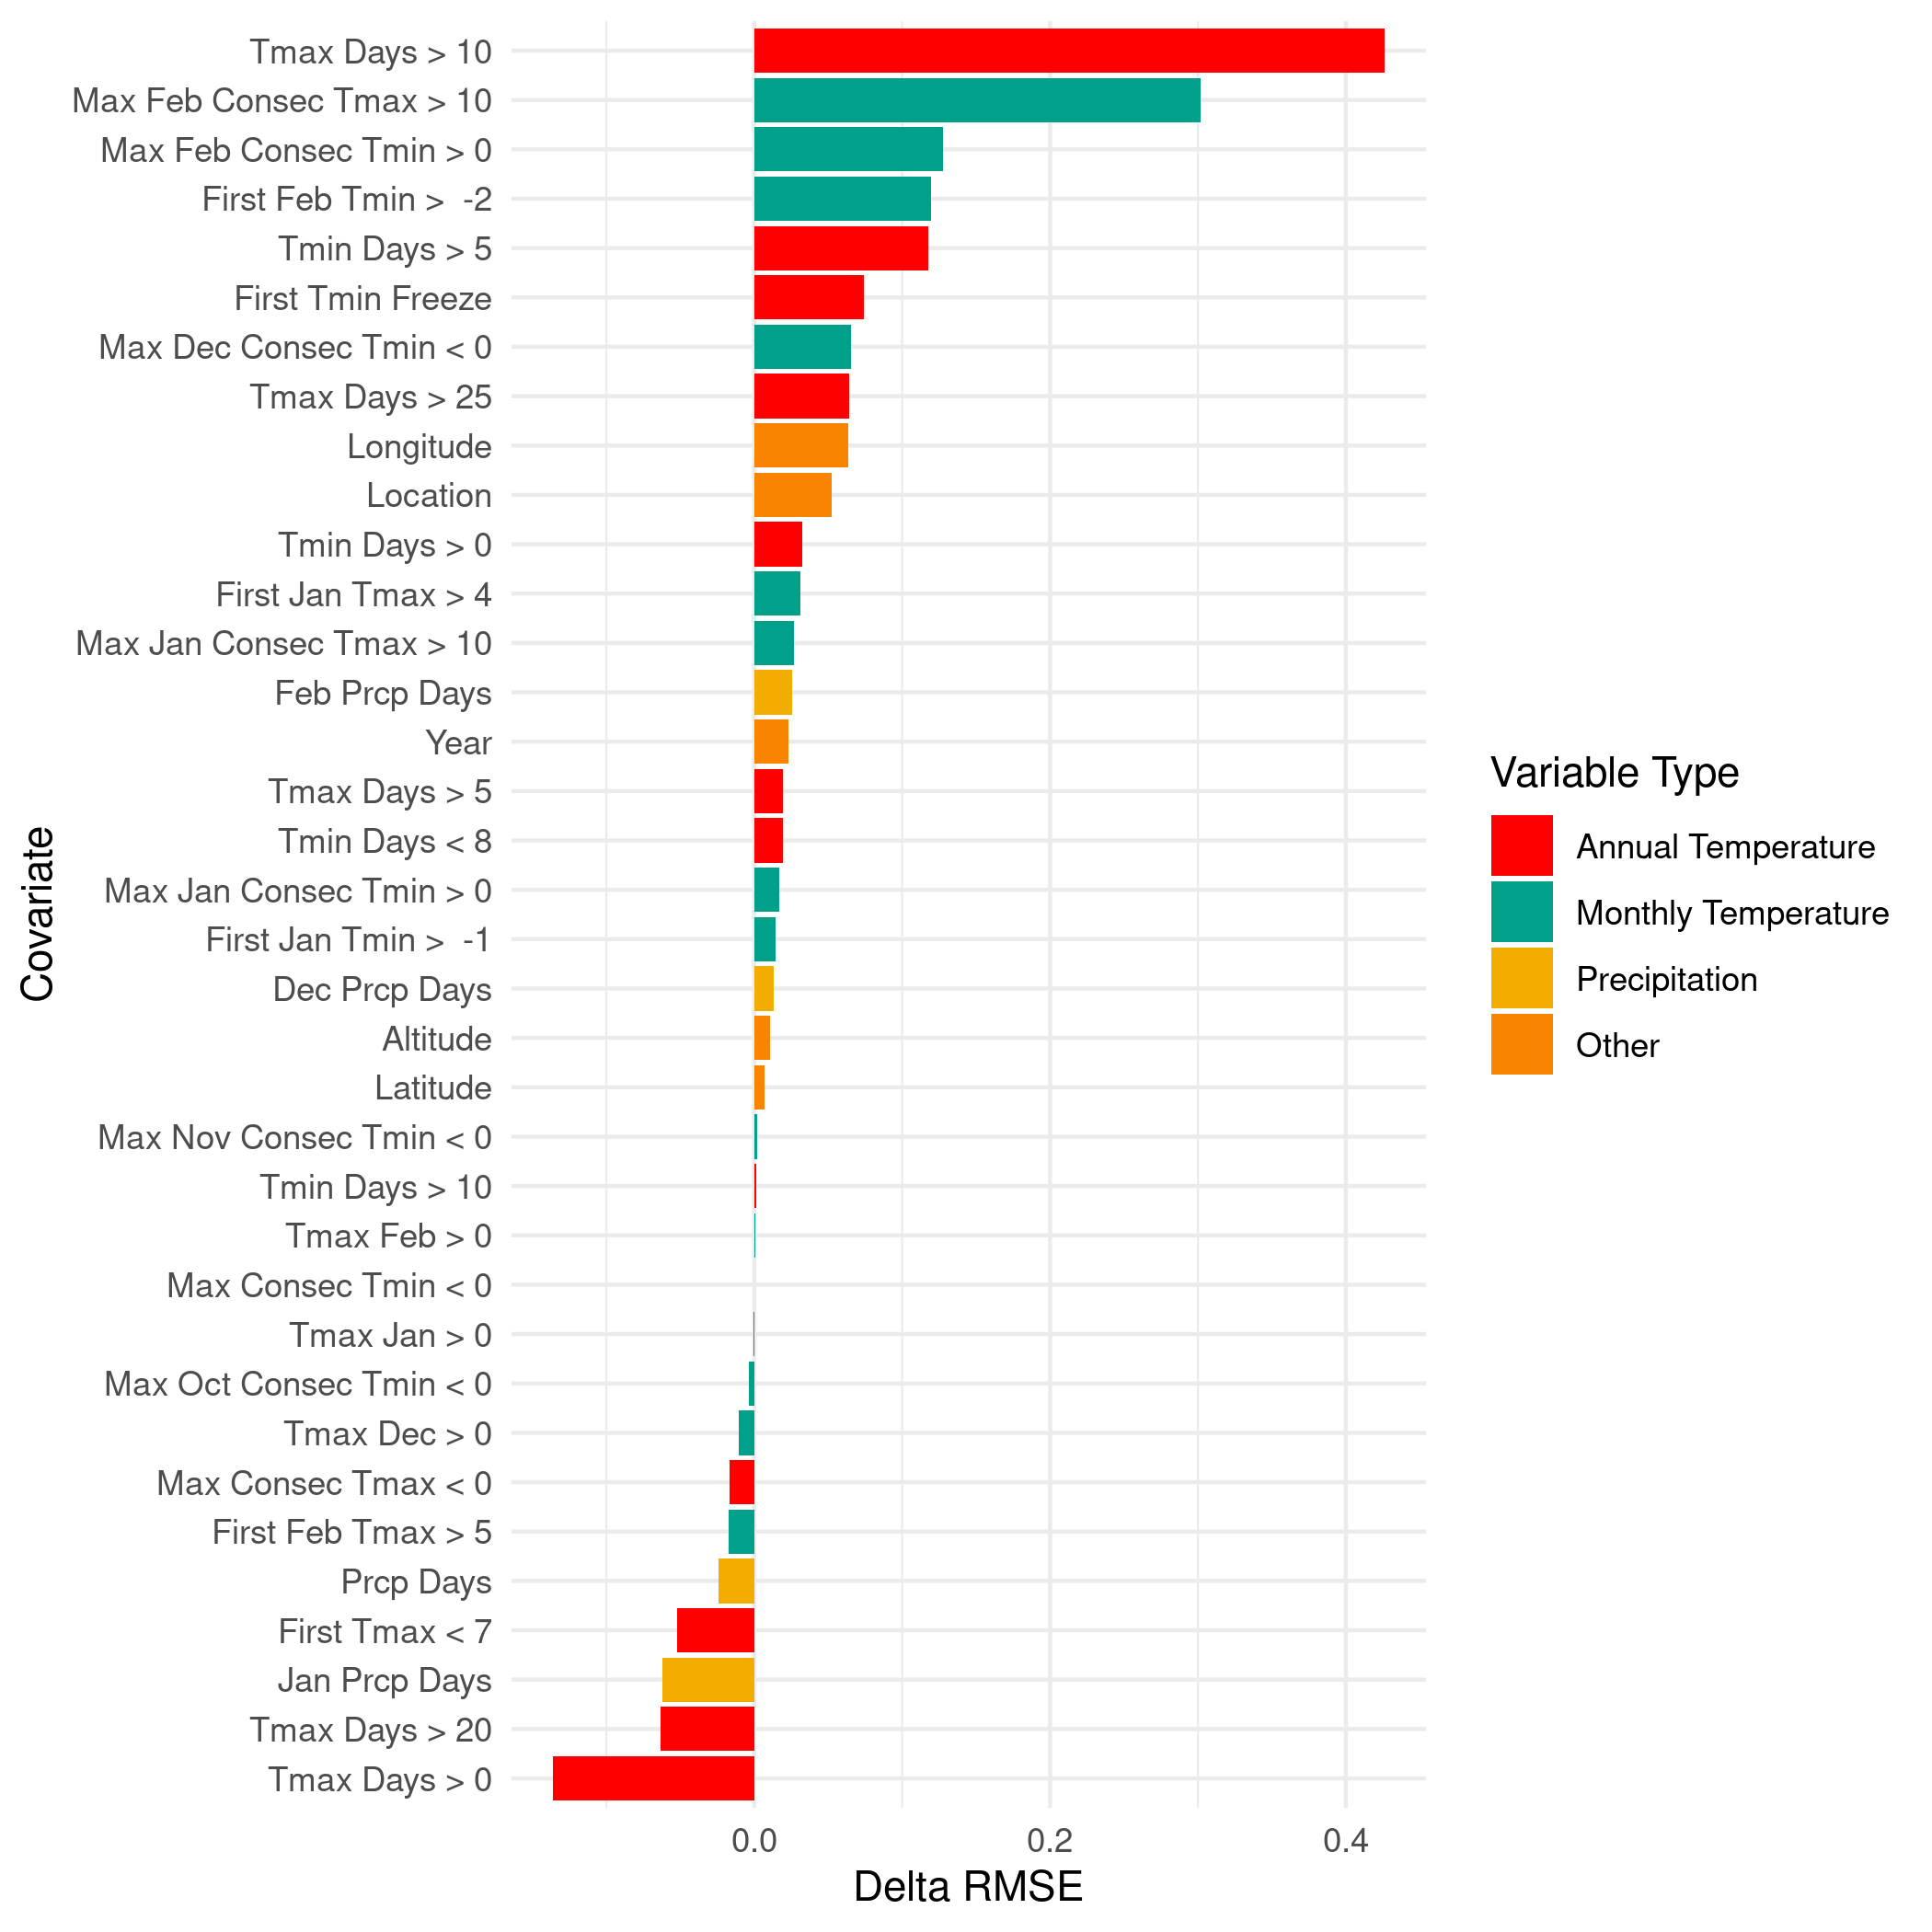
\includegraphics[width=\textwidth]{Figures/variableImportancePlot.png}
  \caption{Ranking of covariate importance for accurate model prediction. Variables are ranked according to their impact on the model's root mean squared error on a holdout set of data; positive values indicate variables that worsen the model's ability to predict and negative values indicate variables that augment the model's ability to predict. Color represents the variable type, either annual temperature, monthly temperature, precipitation, or other.}
  \label{fig:varImportance}
\end{figure}

\clearpage 

\begin{figure}
  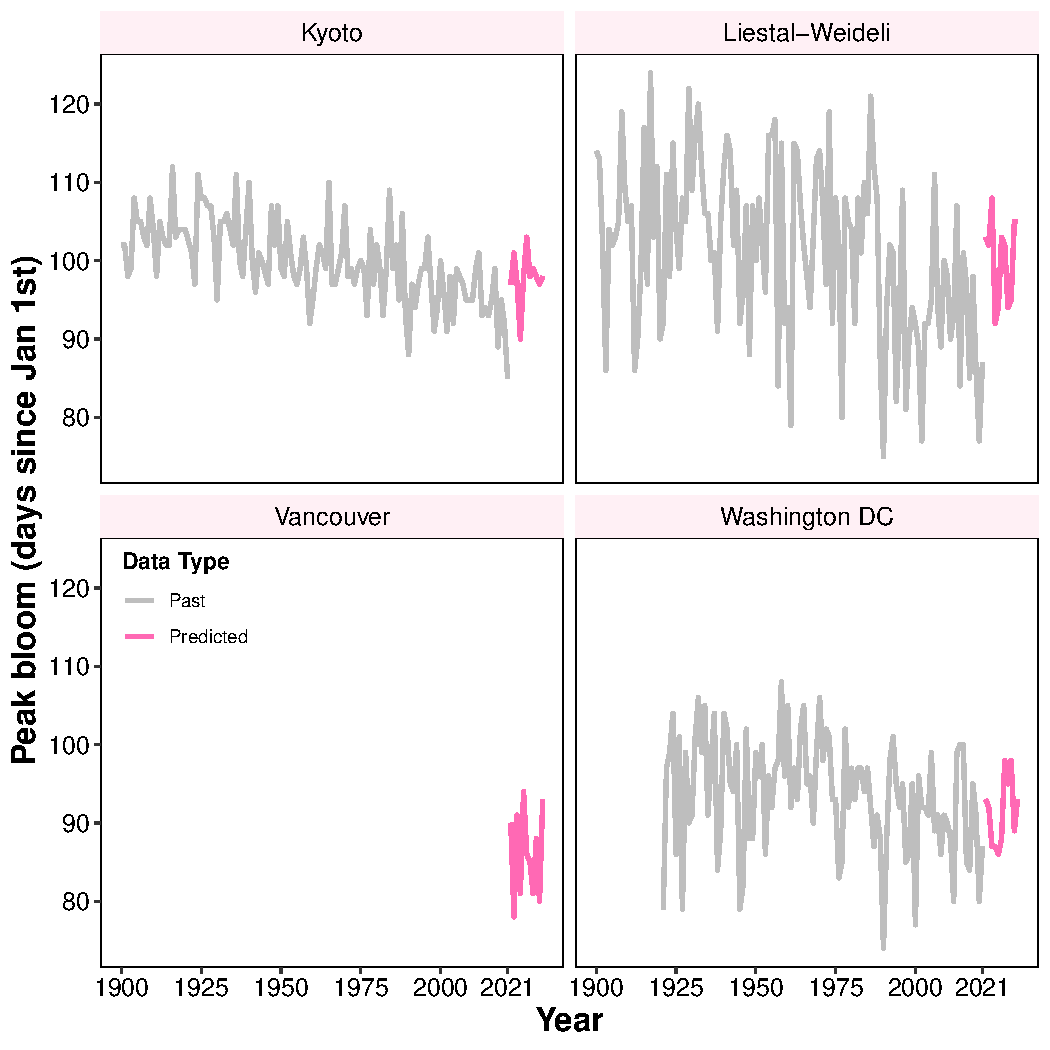
\includegraphics[width=\textwidth]{Figures/time_seriesPlot.pdf}
  \caption{Past and predicted peak bloom dates (days since January 1st) for the competition sites (Kyoto, Liestal−Weideli, Vancouver, Washington DC). Past data are plotted in a gray and have been represented from 1900 to 2021, though for Kyoto the data extends back to 1812 and for Vancouver there is no historic data. Predicted peak bloom dates from the ensemble model are represented in pink for each site spanning 2022-2032.}
  \label{fig:tsPredications}
\end{figure}






\clearpage
\bibliography{bib}
\bibliographystyle{plain}

\end{document}
